
\begin{figure}[ht]
\centering

\begin{subfigure}[b]{0.45\textwidth}
    \centering
    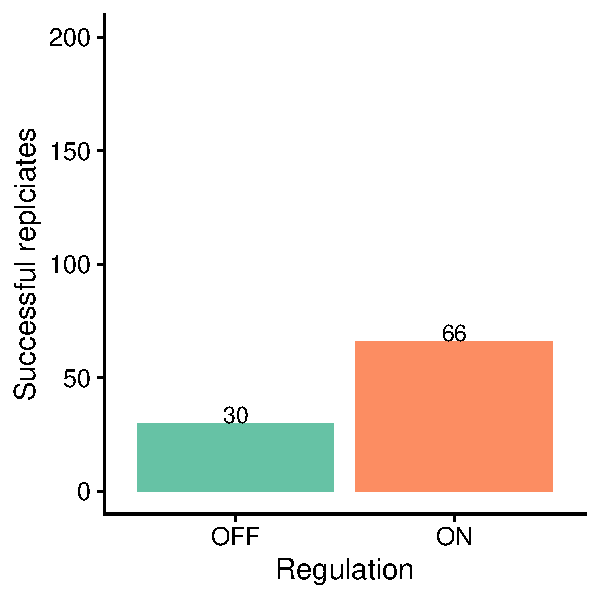
\includegraphics[width=\linewidth]{chapters/05-tag-based-genetic-regulation/media/boolean-calc-prefix-solution-counts.pdf}
    \caption{\small Successful replicates.}
    \label{chapter:tag-based-regulation:subfig:boolean-calc-prefix-solution-count}
\end{subfigure}
\hfill
\begin{subfigure}[b]{0.45\textwidth}
    \centering
    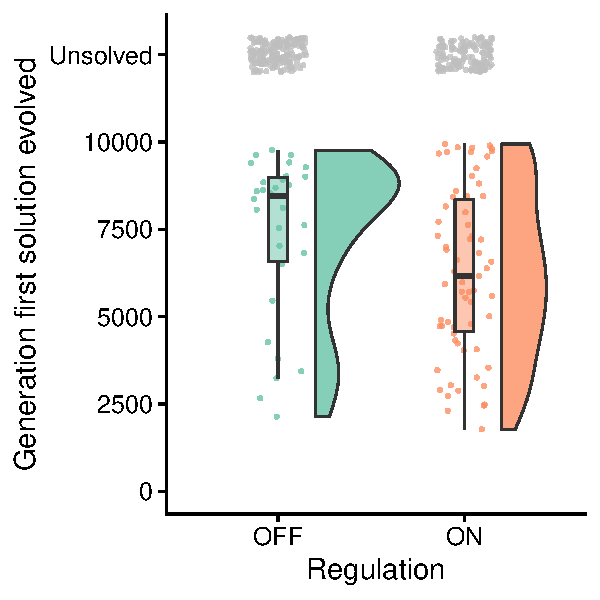
\includegraphics[width=\textwidth]{chapters/05-tag-based-genetic-regulation/media/boolean-calc-prefix-solve-time-cloud.pdf}
    \caption{\small Generations elapsed before solution.}
    \label{chapter:tag-based-regulation:subfig:boolean-calc-prefix-solve-time}
\end{subfigure}

\caption{\small
\textbf{Boolean-logic calculator problem-solving performance.}
(a) shows the number of successful replicates for the regulation-off and regulation-on conditions on the Boolean-logic calculator problem. 
The regulation-off condition was less successful than the regulation-on condition (Fisher's exact test: $p < 4\times10^{-05}$).
(b) is a raincloud plot showing the generation at which the first solution evolved in each successful replicate.
Gray points indicate the number of unsuccessful replicates for each condition.
Regulation-on solutions typically required fewer generations than regulation-off solutions to arise (Wilcoxon rank sum test: $p < 0.042$).
}

% fisher's  p-value = 3.585e-05
% wilcoxon rank sum: p-value = 0.04102
    
\label{chapter:tag-based-regulation:fig:boolean-calc-prefix-performance}
\end{figure}
